% 第8章第1节：给定函数的有限逼近（多项式、样条、核截面、神经网络）。

\section{给定函数的有限逼近}
\label{sec:apx-single-function}

本节固定一个目标函数、它的定义域和衡量误差的范数，再挑选一类生成单元，用它们的有限线性组合去接近目标。主要的误差范数是一致范数$\|f\|_\infty=\sup_x|f(x)|$（第~\ref{sec:fs-uniform-norm}节），它要求整个定义域上的误差同时变小。四小节分别使用多项式、分段直线、固定宽度的高斯核截面和神经单元；每一种都有自己的预算，即次数、结点数、中心个数或单元个数。

贯穿全节的目标是
\[
  f_*(x)=\left|x-\frac12\right|,\qquad x\in[0,1].
\]
它连续，却在$x=1/2$处有折点。后面会看到：多项式只能随次数增加而逼近它，含结点$1/2$的线性样条和两个ReLU单元却能精确表示它。这个对照比较的是同一目标在不同生成规则下需要的条件，不能由一个例子推出某种方案对所有目标都更节省。

读结论时要分清两类陈述。“对每个$\varepsilon>0$，存在某个预算下的近似，误差小于$\varepsilon$”是可变预算下的存在性，预算可以随$\varepsilon$增长；“预算为$m$时误差不超过某个量”是固定预算下的误差保证，通常要求目标满足额外的光滑性。前者回答能否逼近，后者回答逼近得多快。

\subsection{多项式逼近}
\label{sec:apx-polynomial}

多项式是最早被系统研究的逼近工具：给定次数，它由有限个系数确定，求值只需加法和乘法。本小节先构造一列具体的多项式并证明它一致逼近任意连续目标，再把构造中真正用到的性质提炼成一般定理。

\paragraph{连续模}

要估计全区间上的误差，需要一个量来记录目标在小尺度上能变化多少。

\begin{definition}[连续模]
\label{def:apx-modulus-of-continuity}
设$f$是区间$I$上的有界函数。对$\delta>0$，令
\[
  \omega_f(\delta)=\sup\bigl\{|f(s)-f(t)|:\ s,t\in I,\ |s-t|\le\delta\bigr\},
\]
称$\omega_f$为$f$的\term{连续模}（modulus of continuity）。
\end{definition}

连续模关于$\delta$单调不减。$f$在$I$上一致连续，恰好等价于$\omega_f(\delta)\to0$（$\delta\downarrow0$）；在紧区间上，连续函数都一致连续（定理~\ref{thm:metric-compact-uniform}），所以$C([0,1])$中每个函数的连续模都趋于零。若$f$满足$|f(s)-f(t)|\le L|s-t|$，则$\omega_f(\delta)\le L\delta$。

对贯穿目标，$|f_*(s)-f_*(t)|\le|s-t|$；取$s=0$、$t=\delta$（$\delta\le1/2$）时等号成立，而$f_*$的取值在$[0,1/2]$中，因此
\[
  \omega_{f_*}(\delta)=\min\{\delta,1/2\}.
\]
再看$g(x)=\sqrt x$：由$|\sqrt s-\sqrt t|\le\sqrt{|s-t|}$且在$s=0$处取等号，得$\omega_g(\delta)=\sqrt\delta$（$\delta\le1$）。两个函数都连续，但$g$在原点附近变化得更剧烈，连续模下降得更慢。后面的误差界都以连续模表示，这个差别会直接反映在速率上。

\paragraph{Bernstein多项式}

现在构造逼近多项式。固定整数$m\ge1$，在等距结点$j/m$处读取$f$的值，令
\begin{equation}
  B_mf(x)=\sum_{j=0}^{m}f\Bigl(\frac jm\Bigr)w_{m,j}(x),
  \qquad
  w_{m,j}(x)=\binom mj x^j(1-x)^{m-j},
  \label{eq:apx-bernstein}
\end{equation}
称为$f$的$m$次\term{Bernstein多项式}（Bernstein polynomial）\scite{bernstein1912demonstration}。每个权重$w_{m,j}$都是次数为$m$的多项式，所以$B_mf$是次数至多$m$的多项式；系数只需要$m+1$个结点值。

权重有两个直接可见的性质。在$[0,1]$上每个$w_{m,j}(x)\ge0$；由二项式定理，
\[
  \sum_{j=0}^m w_{m,j}(x)=\bigl(x+(1-x)\bigr)^m=1.
\]
因此$B_mf(x)$是结点值的凸组合，取值不会超出结点值的范围。图~\ref{fig:apx-bernstein-approx}画出$f_*$的三个Bernstein多项式：曲线随$m$增大而贴近折线，最大误差都出现在折点处。

\begin{figure}[!htb]
  \centering
  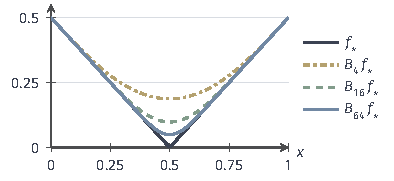
\includegraphics[width=66.7mm]{figures/02-abstract-mathematics/03-function-spaces/tikz/c6-bernstein-approx/figure.pdf}
  \caption{折线$f_*(x)=|x-1/2|$（黑）及其Bernstein多项式$B_4f_*$、$B_{16}f_*$、$B_{64}f_*$。每条曲线都是结点值的凸组合，位于$f_*$上方；一致误差都在$x=1/2$处取得，依次为$0.1875$、$0.0982$、$0.0497$，次数每增至四倍，误差约减半。}
  \label{fig:apx-bernstein-approx}
\end{figure}

凸组合只说明取值范围，还没有说明权重集中在哪些结点上。若权重主要落在离$x$较近的结点，$B_mf(x)$就主要由$f$在$x$附近的值决定。下面的矩恒等式把这个直觉写成精确的计算。

\begin{lemma}[Bernstein权重的矩]
\label{lem:apx-bernstein-moments}
对$0\le x\le1$和$m\ge1$，
\[
  \sum_{j=0}^m j\,w_{m,j}(x)=mx,\qquad
  \sum_{j=0}^m j(j-1)\,w_{m,j}(x)=m(m-1)x^2,
\]
从而
\begin{equation}
  \sum_{j=0}^m\Bigl(\frac jm-x\Bigr)^2w_{m,j}(x)=\frac{x(1-x)}m\le\frac1{4m}.
  \label{eq:apx-bernstein-variance}
\end{equation}
\end{lemma}

\begin{proof}
第一式利用$j\binom mj=m\binom{m-1}{j-1}$。$j=0$的项为零，把下标改为$k=j-1$，
\[
  \sum_{j=0}^m j\,w_{m,j}(x)
  =mx\sum_{k=0}^{m-1}\binom{m-1}{k}x^k(1-x)^{m-1-k}=mx,
\]
最后一步再次使用二项式定理。第二式同理利用$j(j-1)\binom mj=m(m-1)\binom{m-2}{j-2}$，把下标改为$k=j-2$即得；$m=1$时两边都为零。

对中心矩，把$(j/m-x)^2$展开，并用$j^2=j(j-1)+j$：
\[
  \sum_{j}\Bigl(\frac jm-x\Bigr)^2w_{m,j}
  =\frac{m(m-1)x^2+mx}{m^2}-2x\cdot\frac{mx}{m}+x^2
  =\frac{x(1-x)}m .
\]
最后由$x(1-x)\le1/4$得到上界$1/(4m)$。
\end{proof}

式~\eqref{eq:apx-bernstein-variance}说明，以$w_{m,j}(x)$为权重时，结点$j/m$与$x$的平均平方距离只有$x(1-x)/m$。若读者熟悉概率，这些权重正是二项分布$\mathrm{Bin}(m,x)$的概率，上述三式分别是总概率、均值与方差；证明只用到有限和，不依赖概率论。

\paragraph{近邻与远处的误差分解}

有了权重的集中性，就可以把误差分成两部分来控制：近邻结点上$f$的值接近$f(x)$，远处结点的总权重很小。

\begin{theorem}[Bernstein--Weierstrass逼近]
\label{thm:apx-bernstein}
设$f\in C([0,1])$。对每个$m\ge1$和每个$\delta>0$，
\begin{equation}
  \|B_mf-f\|_\infty\le\omega_f(\delta)+\frac{\|f\|_\infty}{2m\delta^2}.
  \label{eq:apx-bernstein-error}
\end{equation}
因此$\|B_mf-f\|_\infty\to0$（$m\to\infty$）。特别地，$[0,1]$上的多项式在$C([0,1])$中一致稠密。
\end{theorem}

\begin{proof}
固定$x\in[0,1]$。由权重和为一，误差可以写成
\[
  B_mf(x)-f(x)=\sum_{j=0}^m\Bigl[f\Bigl(\frac jm\Bigr)-f(x)\Bigr]w_{m,j}(x).
\]
按$|j/m-x|\le\delta$与$|j/m-x|>\delta$把结点分成近邻与远处两组。

近邻组中每个差值的绝对值不超过$\omega_f(\delta)$，而近邻权重之和不超过$1$，所以这一组的贡献至多为$\omega_f(\delta)$。

远处组中每个差值不超过$2\|f\|_\infty$。对远处的结点有$1<(j/m-x)^2/\delta^2$，于是由式~\eqref{eq:apx-bernstein-variance}，
\[
  \sum_{|j/m-x|>\delta}w_{m,j}(x)
  \le\frac1{\delta^2}\sum_{j=0}^m\Bigl(\frac jm-x\Bigr)^2w_{m,j}(x)
  \le\frac1{4m\delta^2},
\]
这一组的贡献至多为$2\|f\|_\infty/(4m\delta^2)$。两组相加后右端不依赖$x$，对$x$取上确界即得式~\eqref{eq:apx-bernstein-error}。

为了得到收敛，次序很重要。任给$\varepsilon>0$，先利用一致连续性选$\delta$使$\omega_f(\delta)<\varepsilon/2$；保持这个$\delta$不变，再取$m$足够大，使$\|f\|_\infty/(2m\delta^2)<\varepsilon/2$。若先固定$m$再缩小$\delta$，第二项会变大，论证不能成立。
\end{proof}

图~\ref{fig:apx-bernstein-weights}以$m=50$、$x=0.3$、$\delta=0.15$为例画出全部权重。蓝色的近邻结点占去权重$0.980$，黄色的远处结点只有$0.020$；矩估计给出的远处权重上界为$x(1-x)/(m\delta^2)=0.187$，再放大为$1/(4m\delta^2)=0.222$。上界相当保守，但它不依赖$x$，这正是全区间共用的误差界所需要的。

\begin{figure}[!htb]
  \centering
  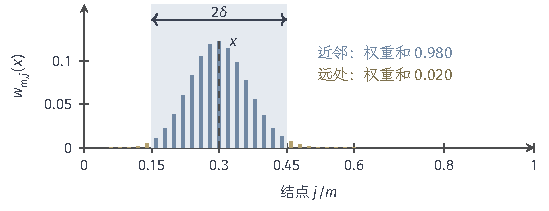
\includegraphics[width=93.0mm]{figures/02-abstract-mathematics/03-function-spaces/tikz/c6-bernstein-weights/figure.pdf}
  \caption{Bernstein权重的集中性：$m=50$、$x=0.3$时各结点$j/m$上的权重$w_{m,j}(x)$。蓝底为近邻窗口$|j/m-x|\le\delta=0.15$，窗口内权重和为$0.980$，窗口外（黄色）仅$0.020$。误差分解中，近邻部分由连续模$\omega_f(\delta)$控制，远处部分由二阶中心矩$x(1-x)/m$控制。}
  \label{fig:apx-bernstein-weights}
\end{figure}

\paragraph{折点目标与收敛速度}

定理~\ref{thm:apx-bernstein}保证$f_*$可以被多项式任意逼近，但任何一个多项式都不等于$f_*$：多项式处处可微，而$f_*$在$1/2$处的左右导数分别为$-1$和$1$。“可以任意逼近”与“能被某个有限次多项式精确表示”是两回事。

收敛有多快取决于目标的正则性。若$f$是$L$-Lipschitz的，可以不经过近远分解，直接用Cauchy--Schwarz不等式估计：
\[
  |B_mf(x)-f(x)|
  \le L\sum_{j}\Bigl|\frac jm-x\Bigr|w_{m,j}(x)
  \le L\Bigl(\sum_j\Bigl(\frac jm-x\Bigr)^2w_{m,j}(x)\Bigr)^{1/2}
  \le\frac{L}{2\sqrt m}.
\]
对$f_*$，$L=1$，这个界在$m=4,16,64$时分别为$0.25$、$0.125$、$0.0625$，实际误差$0.1875$、$0.0982$、$0.0497$与它同阶。对$\sqrt x$只有$|f(s)-f(t)|\le|s-t|^{1/2}$，同样的论证（先对$|j/m-x|^{1/2}$用Cauchy--Schwarz）只给出$(4m)^{-1/4}$。条件越弱，这个构造能保证的速率越慢。

Bernstein多项式也不是相应次数下最好的多项式。由引理~\ref{lem:apx-bernstein-moments}，
\[
  B_m(x^2)=\frac{m(m-1)x^2+mx}{m^2}=x^2+\frac{x(1-x)}m,
\]
所以对$x^2$本身，误差恰为$1/(4m)$，而$x^2$只是一个二次多项式。这个构造的价值在于每一步都可以验证，并给出所有连续函数共同的收敛机制；最佳逼近的误差需要另外研究。

\paragraph{Stone--Weierstrass定理}

回看定理~\ref{thm:apx-bernstein}的结论：$[0,1]$上的多项式在一致范数下稠密。把多项式换成其他函数族、把区间换成其他紧集时，哪些性质仍然是关键？多项式族对加法、数乘和乘法封闭，含有常数，而且函数$x$能区分任意两个不同的点。下面的定理说明这几条已经足够。

设$K$是非空紧度量空间，$C(K)$为$K$上全体实值连续函数，配备一致范数。若子空间$\mathcal A\subseteq C(K)$对逐点乘法封闭，就称它是\term{子代数}（subalgebra）；若对任意$x\ne y$都有$h\in\mathcal A$使$h(x)\ne h(y)$，就称$\mathcal A$\term{分离点}（separates points）。

\begin{theorem}[Stone--Weierstrass定理]
\label{thm:apx-stone-weierstrass}
设$K$是非空紧度量空间，$\mathcal A\subseteq C(K)$是含有常数函数且分离点的子代数，则$\mathcal A$在$C(K)$中按一致范数稠密：对每个$f\in C(K)$和$\varepsilon>0$，存在$h\in\mathcal A$使$\|f-h\|_\infty<\varepsilon$。
\end{theorem}

这一结论由Stone对Weierstrass多项式逼近定理的推广给出\scite{stone1948generalized}。它立即覆盖多变量的情形：在紧集$K\subset\mathbb R^d$上，$d$元多项式组成含常数的子代数，坐标函数分离点，因此多元多项式在$C(K)$中稠密。另一个例子是单位圆周：把$[0,2\pi]$的两端看成同一点，三角多项式$\sum_{k=0}^n(a_k\cos kt+b_k\sin kt)$对乘法封闭（由积化和差），含有常数，$\cos t$与$\sin t$合起来分离圆周上的点，因此在圆周上的连续函数中稠密。

两个条件各自不可缺少。在$[-1,1]$上，偶多项式组成含常数的子代数，但对每个偶多项式都有$p(x)=p(-x)$，它不能分离$x$与$-x$；一致极限仍是偶函数，因此奇函数$x$不在闭包中。在$[0,1]$上，满足$p(0)=0$的多项式组成分离点的子代数，但不含常数；一致极限都在$0$处取零，所以常函数$1$不在闭包中。

\begin{proof}[补充阅读：证明思路]
记$\overline{\mathcal A}$为一致闭包，它仍是含常数的子代数。第一步，若$h\in\overline{\mathcal A}$，则$|h|\in\overline{\mathcal A}$：在$[-\|h\|_\infty,\|h\|_\infty]$上用多项式$p$一致逼近$|t|$（定理~\ref{thm:apx-bernstein}经线性变量代换），$p\circ h$属于$\overline{\mathcal A}$且一致接近$|h|$。由$\max\{g,h\}=(g+h+|g-h|)/2$和$\min\{g,h\}=(g+h-|g-h|)/2$，$\overline{\mathcal A}$对有限个函数取最大、最小封闭。第二步，由分离点和常数，对任意$x\ne y$和实数$a,b$，存在$h\in\mathcal A$满足$h(x)=a$、$h(y)=b$：取$u$使$u(x)\ne u(y)$，令$h=a+(b-a)(u-u(x))/(u(y)-u(x))$。第三步，固定$f$、$\varepsilon$和$x$，对每个$y$取$h_y$使$h_y(x)=f(x)$、$h_y(y)=f(y)$；集合$\{z:h_y(z)<f(z)+\varepsilon\}$是开集并覆盖$K$，由紧性取有限个，令$g_x=\min h_{y_i}$，则$g_x<f+\varepsilon$且$g_x(x)=f(x)$。再对开集$\{z:g_x(z)>f(z)-\varepsilon\}$用一次紧性，取有限个$g_{x_k}$的最大值，即得$\overline{\mathcal A}$中与$f$一致误差小于$\varepsilon$的函数。
\end{proof}

\paragraph{稠密性与误差速率}

Stone--Weierstrass定理只回答“能否任意逼近”，不提供任何速率：它没有说明达到精度$\varepsilon$需要多少项，证明中的紧性步骤也不给出项数。定理~\ref{thm:apx-bernstein}之所以能给出速率，是因为对目标另加了连续模或Lipschitz常数等定量条件。要比较不同生成单元的效率，必须先固定这样一个函数类；第~\ref{sec:apx-function-classes}节将把“固定一个函数类”本身作为研究对象。

\subsection{样条逼近}
\label{sec:apx-splines}

多项式是全局的：改变一个系数，整个区间上的函数值都会改变，Bernstein权重也在整个$(0,1)$上非零。另一种思路是把区间切成小段，每段只用低次多项式，段与段之间按一定光滑性衔接。这类分段多项式称为\term{样条}（spline），分段的位置称为\term{结点}（knot）。本小节从最简单的连续分段直线开始。

\paragraph{线性插值与连续模界}

固定结点$0=t_0<t_1<\cdots<t_N=1$，记最大间距$h=\max_i(t_{i+1}-t_i)$。对$x\in[t_i,t_{i+1}]$，令
\begin{equation}
  S_hf(x)=(1-s)f(t_i)+s\,f(t_{i+1}),\qquad s=\frac{x-t_i}{t_{i+1}-t_i}\in[0,1].
  \label{eq:apx-linear-interpolant}
\end{equation}
相邻两段在公共结点取同一个值，所以$S_hf$是经过全部结点值的连续折线，称为$f$的线性插值。全体在每段上为一次函数的连续函数组成\term{线性样条}（linear spline）空间，它是$N+1$维的线性空间；$S_h$则是从结点值产生其中一个元素的操作。图~\ref{fig:apx-spline-hat}(a)画出一个光滑函数在七个等距结点上的线性插值。

\begin{theorem}[线性插值的误差]
\label{thm:apx-linear-interpolation}
在上述记号下，若$f\in C([0,1])$，则
\begin{equation}
  \|f-S_hf\|_\infty\le\omega_f(h).
  \label{eq:apx-spline-modulus}
\end{equation}
若进一步$f\in C^2([0,1])$，则
\begin{equation}
  \|f-S_hf\|_\infty\le\frac{h^2}{8}\|f''\|_\infty .
  \label{eq:apx-spline-quadratic}
\end{equation}
\end{theorem}

\begin{proof}
先证连续模界。在单元$[t_i,t_{i+1}]$上，利用$(1-s)+s=1$，
\[
  f(x)-S_hf(x)=(1-s)\bigl(f(x)-f(t_i)\bigr)+s\bigl(f(x)-f(t_{i+1})\bigr).
\]
$x$到两个端点的距离都不超过$h$，所以两个差值都不超过$\omega_f(h)$，凸组合也不超过$\omega_f(h)$。对所有单元取上确界即得式~\eqref{eq:apx-spline-modulus}。

再证二阶界。固定单元和其中一点$x\in(t_i,t_{i+1})$，令$g=f-S_hf$，它在两端为零。取
\[
  \lambda=\frac{g(x)}{(x-t_i)(x-t_{i+1})},\qquad
  G(u)=g(u)-\lambda(u-t_i)(u-t_{i+1}),
\]
则$G$在$t_i$、$x$、$t_{i+1}$三点为零。两次使用Rolle定理，存在$\xi\in(t_i,t_{i+1})$使$G''(\xi)=0$。由于$S_hf$在单元内是一次函数，$G''(\xi)=f''(\xi)-2\lambda$，故$\lambda=f''(\xi)/2$，即
\[
  f(x)-S_hf(x)=\frac{f''(\xi)}2(x-t_i)(x-t_{i+1}).
\]
在单元上$|(x-t_i)(x-t_{i+1})|\le(t_{i+1}-t_i)^2/4\le h^2/4$，代入即得式~\eqref{eq:apx-spline-quadratic}。
\end{proof}

两个界依据不同。连续模界只用了凸组合，对任何连续目标成立，并且不要求结点等距：只要一列网格的最大间距$h\to0$，插值就一致收敛到$f$。二阶界多用了$f''$的有界性，换来$h^2$的速率；Rolle定理与插值余项可参考\BookChapterRef{chap:univariate-differentiation}{卷一“一元函数的微分”章}。

二阶界中的常数$1/8$不能改进。取$f(x)=x^2$，只用两个结点$0$和$1$，则$S_hf(x)=x$，误差$x-x^2$在$x=1/2$处取最大值$1/4$；此时$h=1$、$\|f''\|_\infty=2$，右端$h^2\|f''\|_\infty/8=1/4$，等号成立。

\paragraph{额外光滑性带来的速率}

二阶速率所用的光滑性不能省略。取等距结点$t_i=i/N$，$N$为奇数，此时$1/2$不是结点，而落在单元$[(N-1)/(2N),(N+1)/(2N)]$的中点。$f_*$在这个单元的两个端点取值都是$h/2$，插值在单元内恒为$h/2$，而$f_*(1/2)=0$；其余单元上$f_*$本身就是直线，插值没有误差。因此$\|f_*-S_hf_*\|_\infty=h/2$，只按一阶下降，这与$\omega_{f_*}(h)=h$的界同阶。

图~\ref{fig:apx-spline-rates}在对数坐标中比较两种目标。光滑函数$\sin(\pi x)$的实测误差几乎落在二阶界$\pi^2h^2/8$上，斜率为$2$；$f_*$的误差落在直线$h/2$上，斜率为$1$。网格宽度控制的是表示的分辨率，同一分辨率下能达到的精度取决于目标的光滑性。

\begin{figure}[!htb]
  \centering
  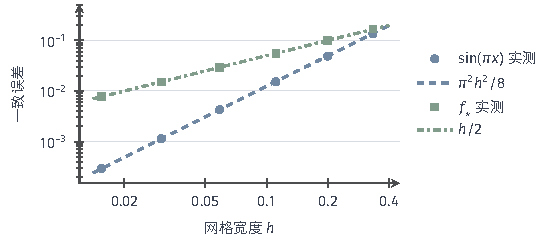
\includegraphics[width=93.4mm]{figures/02-abstract-mathematics/03-function-spaces/tikz/c6-spline-rates/figure.pdf}
  \caption{等距线性插值的一致误差与网格宽度$h=1/N$（$N=3,5,\ldots,65$为奇数，$1/2$不是结点），双对数坐标。光滑目标$\sin(\pi x)$的误差（圆点）贴近二阶界$\pi^2h^2/8$；折线$f_*$的误差（方块）恰为$h/2$，只按一阶下降。}
  \label{fig:apx-spline-rates}
\end{figure}

\paragraph{帽形基与局部修改}

线性插值可以改写成固定基函数的线性组合。对每个结点$t_i$，令$\varphi_i$为在$t_i$处取$1$、在其余结点处取$0$的线性样条；它在$[t_{i-1},t_{i+1}]$上呈三角形，在别处为零，称为\term{帽形函数}（hat function）。于是
\[
  S_hf=\sum_{i=0}^{N}f(t_i)\varphi_i,\qquad \sum_{i=0}^N\varphi_i\equiv1 .
\]
系数恰好是结点值，基函数非负且和为一，这正是式~\eqref{eq:apx-linear-interpolant}中凸组合的来源。

若结点包含$1/2$，例如取$t_0=0$、$t_1=1/2$、$t_2=1$，则$f_*$在每段上都是直线，
\[
  f_*=\tfrac12\varphi_0+0\cdot\varphi_1+\tfrac12\varphi_2 ,
\]
三个系数就精确表示了它。这比任何次数的多项式都节省，原因在于结点恰好放在折点上；同一组结点并不能精确表示任意连续目标。

帽形基的支撑只覆盖相邻两段，因此修改一个结点值只影响局部。图~\ref{fig:apx-spline-hat}(b)把$t_3=1/2$处的值由$0.5$改为$0.8$，插值只在$[t_2,t_4]=[1/3,2/3]$上改变。这里有两个不同来源的性质：局部性来自基函数的支撑，误差界来自凸组合；后面换用其他基时，需要分别重新检查。

\begin{figure}[!htb]
  \centering
  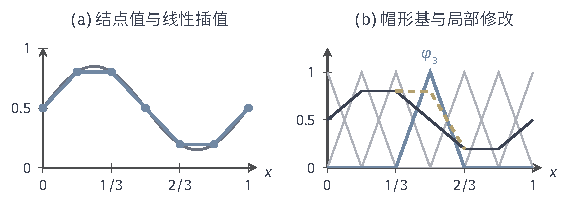
\includegraphics[width=96.2mm]{figures/02-abstract-mathematics/03-function-spaces/tikz/c6-spline-hat/figure.pdf}
  \caption{线性样条与帽形基，结点$t_i=i/6$。(a)~目标$0.5+0.35\sin(2\pi x)$（灰）及其线性插值（蓝折线），圆点为结点值。(b)~七个帽形函数（细灰），其中$\varphi_3$加粗；黑色折线为(a)中的插值，把$t_3$处的结点值改为$0.8$后得到黄色虚线，变化只发生在$\varphi_3$的支撑$[1/3,2/3]$上。}
  \label{fig:apx-spline-hat}
\end{figure}

\paragraph{高次样条与系数恢复}

把每段的一次函数换成$k$次多项式，并要求在内部结点处$k-1$阶导数连续，就得到$k$次样条。$N$段各有$k+1$个系数，每个内部结点施加$k$个衔接条件，空间维数为$(k+1)N-k(N-1)=N+k$。常用的三次样条维数为$N+3$，而结点值只提供$N+1$个条件，还需补充两个端点条件，插值才唯一。

更高的次数和衔接阶带来更光滑的近似，代价是系数与结点值不再直接对应。以等距结点上的三次B样条$\beta_3$为例（$\beta_3(0)=2/3$，$\beta_3(\pm1)=1/6$，在$|s|\ge2$处为零），若$S(x)=\sum_jc_j\beta_3(x-j)$，则在整数结点处
\[
  S(i)=\frac{c_{i-1}+4c_i+c_{i+1}}6 .
\]
要让$S$经过给定的结点值，必须先解这个线性方程组恢复系数；直接把结点值当系数，得到的是相邻值的加权平均。因此要分清三件事：样条空间是哪个候选集合，插值条件从中挑出哪个元素，系数又如何从样本求出。图像重采样中的插值核、预滤波和边界延拓属于信号处理的具体问题，可参考\BookChapterRef{chap:signal-analysis}{卷三“信号”章}。

\subsection{核截面逼近}
\label{sec:apx-kernel-sections}

第~\ref{chap:rkhs}章从半正定核$K$构造了再生核Hilbert空间$H_K$，并证明核截面$K_x=K(\cdot,x)$的有限线性组合在$H_K$中按核范数稠密（第~\ref{sec:rkhs-from-kernel}节）。本小节把核截面当作生成单元，问：在$H_K$之外，有限核和能否逼近更一般的连续目标？

\paragraph{核空间内与核空间外}

先说明核范数下的逼近在什么意义上已经是一致逼近。由再生关系$f(x)=\langle f,K_x\rangle_{H_K}$和Cauchy--Schwarz不等式，$|f(x)|\le\sqrt{K(x,x)}\,\|f\|_{H_K}$（第~\ref{sec:rkhs-kernel-properties}节）。若$\sup_xK(x,x)<\infty$，则$\|f\|_\infty\le\sup_x\sqrt{K(x,x)}\,\|f\|_{H_K}$，核范数下的逼近自动是一致逼近。

本小节固定$[0,1]$上宽度为$\sigma>0$的高斯核
\[
  K_\sigma(x,c)=\exp\Bigl(-\frac{(x-c)^2}{2\sigma^2}\Bigr),
\]
它满足$K_\sigma(x,x)=1$，所以$\|f\|_\infty\le\|f\|_{H_K}$。问题在于$f_*$不属于这个$H_K$。原因是$H_K$中的函数都可微。由再生关系，两个差商$(K_{x+t}-K_x)/t$与$(K_{x+t'}-K_x)/t'$的内积等于
\[
  \frac{K(x+t,x+t')-K(x+t,x)-K(x,x+t')+K(x,x)}{tt'},
\]
$K_\sigma$二阶连续可微，$t,t'\to0$时它趋于$\partial_1\partial_2K(x,x)$。于是差商之差的范数平方$\|(K_{x+t}-K_x)/t-(K_{x+t'}-K_x)/t'\|_{H_K}^2$趋于零，差商在完备空间$H_K$中收敛到某个$D_x$；于是对$f\in H_K$，
\[
  \frac{f(x+t)-f(x)}t=\Bigl\langle f,\frac{K_{x+t}-K_x}t\Bigr\rangle_{H_K}\to\langle f,D_x\rangle_{H_K},
\]
$f$在$x$处可导。$f_*$在$1/2$处不可导，所以$f_*\notin H_K$，第~\ref{chap:rkhs}章的稠密性结论不能直接用于它。

\paragraph{中心差分与加权多项式}

证明的思路是借助多项式。先固定中心$c_0=1/2$，令$w(x)=K_\sigma(x,c_0)$。对中心求导，$\partial_cK_\sigma(x,c)=(x-c)K_\sigma(x,c)/\sigma^2$，每求一次导就多出一个关于$x$的一次因子。由归纳法，
\begin{equation}
  \partial_c^jK_\sigma(x,c_0)=w(x)P_j(x),
  \label{eq:apx-gaussian-derivative}
\end{equation}
其中$P_j$是$j$次多项式，最高次项系数为$\sigma^{-2j}$。归纳步骤是：对$K_\sigma(x,c)Q(x-c)$再关于$c$求导，得到$K_\sigma(x,c)\bigl[(x-c)Q(x-c)/\sigma^2-Q'(x-c)\bigr]$，第一项把次数提高一次并把首项系数乘以$\sigma^{-2}$，第二项次数更低。

导数本身还不是有限核和，需要用差分代替。对固定的$j$和步长$t>0$，中心$j$阶前向差分
\begin{equation}
  D_t^{(j)}(x)=t^{-j}\sum_{\ell=0}^{j}(-1)^{j-\ell}\binom j\ell K_\sigma(x,c_0+\ell t)
  \label{eq:apx-center-difference}
\end{equation}
是$j+1$个核截面的线性组合。反复使用微积分基本定理，可以把它写成导数的平均：
\[
  D_t^{(j)}(x)=t^{-j}\int_0^t\!\!\cdots\!\int_0^t\partial_c^jK_\sigma(x,c_0+u_1+\cdots+u_j)\,\mathrm du_1\cdots\mathrm du_j .
\]
积分中的中心都落在$[c_0,c_0+jt]$内。$\partial_c^jK_\sigma$在紧矩形$[0,1]\times[c_0,c_0+1]$上一致连续，所以
\[
  \begin{aligned}
  \sup_{x\in[0,1]}\bigl|D_t^{(j)}(x)-w(x)P_j(x)\bigr|
  &\le\sup_{x\in[0,1],\ 0\le u\le jt}\bigl|\partial_c^jK_\sigma(x,c_0+u)-\partial_c^jK_\sigma(x,c_0)\bigr|\\
  &\to0\qquad(t\downarrow0).
  \end{aligned}
\]
一致性来自这里的二元一致连续，逐点求导本身只给出每个$x$处的收敛。图~\ref{fig:apx-gaussian-sections}(b)画出$j=1$的情形：$t=0.1$时差分与导数的一致偏差为$2.14$，$t=0.02$时降为$0.44$。

\paragraph{高斯核截面的一致稠密性}

有了每个$wP_j$都能由有限核和一致逼近，剩下的工作是把任意连续目标化成$w$乘一个多项式。

\begin{theorem}[固定宽度高斯核截面的一致稠密性]
\label{thm:apx-gaussian-dense}
固定$\sigma>0$。全体有限和$\sum_{\ell=1}^{M}a_\ell K_\sigma(\cdot,c_\ell)$（$M\in\mathbb N$、$a_\ell\in\mathbb R$、$c_\ell\in\mathbb R$均可随目标和精度变化）在$C([0,1])$中按一致范数稠密。
\end{theorem}

\begin{proof}
设$f\in C([0,1])$，$\varepsilon>0$。

第一步，把目标化成加权多项式。$w$在$[0,1]$上连续且有正下界，所以$f/w\in C([0,1])$。由定理~\ref{thm:apx-bernstein}，存在多项式$P$使$\|f/w-P\|_\infty<\varepsilon/2$；由$0<w\le1$，得$\|f-wP\|_\infty<\varepsilon/2$。

第二步，把$P$写成$P_0,\ldots,P_n$的组合，其中$n=\deg P$。$P_j$的首项系数$\sigma^{-2j}\ne0$，所以从$1,x,\ldots,x^n$到$P_0,\ldots,P_n$的系数矩阵是对角元非零的三角矩阵，可逆。因此$P=\sum_{j=0}^nb_jP_j$，$wP=\sum_jb_jwP_j$。

第三步，对每个$j$用差分代替$wP_j$。由上一段的一致收敛，可选步长$t_j$使$\|D_{t_j}^{(j)}-wP_j\|_\infty<\varepsilon/\bigl(2(n+1)(|b_j|+1)\bigr)$。于是$g=\sum_jb_jD_{t_j}^{(j)}$是有限个高斯核截面的线性组合，且
\[
  \|f-g\|_\infty\le\|f-wP\|_\infty+\sum_{j=0}^n|b_j|\,\|wP_j-D_{t_j}^{(j)}\|_\infty<\varepsilon.
\]
\end{proof}

图~\ref{fig:apx-gaussian-sections}(a)取$\sigma=0.15$，在$M$个等距中心处插值$f_*$：$M=5$时一致误差为$0.061$，$M=9$时为$0.024$。这只是一种具体的选系数方式，并不是定理证明中的构造。

\begin{figure}[!htb]
  \centering
  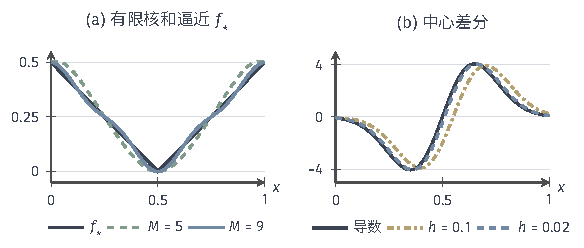
\includegraphics[width=98.9mm]{figures/02-abstract-mathematics/03-function-spaces/tikz/c6-gaussian-sections/figure.pdf}
  \caption{固定宽度$\sigma=0.15$的高斯核截面。(a)~在等距中心$c_\ell=(\ell-1)/(M-1)$处插值$f_*$的有限核和，$M=5$（虚线）与$M=9$（实线），一致误差分别为$0.061$与$0.024$。(b)~中心差分$(K_\sigma(x,\frac12+t)-K_\sigma(x,\frac12))/t$随$t$减小一致逼近导数$(x-\frac12)K_\sigma(x,\frac12)/\sigma^2$，这是一个加权一次多项式。}
  \label{fig:apx-gaussian-sections}
\end{figure}

\paragraph{两种稠密性与结论的条件}

现在可以区分两个命题。第~\ref{chap:rkhs}章的结论是：核截面的有限和在$H_K$中按核范数稠密，它只涉及$H_K$内部的函数。定理~\ref{thm:apx-gaussian-dense}则是：有限核和在$C([0,1])$中按一致范数稠密，它涉及$H_K$之外的目标，例如$f_*$。紧度量空间$X$上的连续核若使$H_K$在$C(X)$中稠密，就称为\term{通用核}（universal kernel）。由于$\|g\|_\infty\le\sup_x\sqrt{K(x,x)}\,\|g\|_{H_K}$，$H_K$中每个元素都能被有限核和一致逼近，所以“$H_K$在$C(X)$中稠密”与“有限核和在$C(X)$中稠密”是同一回事。Steinwart证明了高斯核在$\mathbb R^d$的任意紧子集上都是通用核\cite{steinwart2001kernel}；上面给出的是一维区间上的一条具体证明路线。

定理的条件同样需要逐条读清。

第一，中心、项数和系数都允许随目标与精度变化。若只允许一组预先固定的有限中心，得到的是$C([0,1])$中的有限维子空间；有限维子空间是闭的且不是全空间，不可能稠密。

第二，定理没有对系数或核范数设统一预算。第~\ref{sec:apx-arzela-ascoli}节将证明，核范数不超过$R$的函数组成$C([0,1])$中的紧集，因而是闭集；它只含$H_K$中的函数，所以不含$f_*$，$f_*$到它的一致距离为正。由此，逼近$f_*$的有限核和的核范数必然随精度趋于无穷。

第三，存在性证明不提供数值稳定的选系数方法。差分中出现因子$t^{-j}$，系数会随精度变大；朴素插值也有同样的问题：$\sigma=0.15$时，$M=13$个等距中心的插值误差为$0.023$，最大系数约为$415$；$M=17$时最大系数约为$1.06\times10^6$，误差反而升到$0.097$。如何在给定数据和惩罚下稳定地确定系数，属于后续优化与拟合问题。

\subsection{神经网络逼近}
\label{sec:apx-neural}

神经单元先对输入作仿射变换，再送入一个固定的一元函数，即激活函数；网络的输出是若干单元的线性组合。本小节从一维的分段线性构造开始，把它和样条联系起来，再陈述一般的通用逼近定理。

\paragraph{ReLU单元与折点目标}

\term{整流线性单元}（rectified linear unit，ReLU）使用激活函数$\rho(s)=\max\{s,0\}$。一个单元$x\mapsto a\rho(wx+b)$在$x=-b/w$处折一次，一侧为零，另一侧为斜率$aw$的直线。对贯穿目标，直接验证
\[
  f_*(x)=\rho\Bigl(x-\frac12\Bigr)+\rho\Bigl(\frac12-x\Bigr):
\]
当$x\ge1/2$时第一项为$x-1/2$、第二项为零；当$x\le1/2$时第一项为零、第二项为$1/2-x$。两个单元的输入权重符号相反，偏置都把折点放在$1/2$，输出直接相加，见图~\ref{fig:apx-relu-units}(a)。这个表示由两侧的计算验证，与训练过程无关。

\paragraph{线性样条的ReLU分解}

每个ReLU单元贡献一个折点，这提示连续折线都可以用ReLU单元写出。设连续函数$f$在$[t_0,t_N]$上以$t_0<t_1<\cdots<t_N$为结点分段线性，第$k$段$[t_k,t_{k+1}]$上的斜率为$s_k$。则
\begin{equation}
  f(x)=f(t_0)+s_0(x-t_0)+\sum_{k=1}^{N-1}(s_k-s_{k-1})\rho(x-t_k),\qquad x\in[t_0,t_N].
  \label{eq:apx-relu-spline}
\end{equation}
验证只需比较两侧：右端在$x=t_0$处等于$f(t_0)$，是连续折线；在第$k$段内部，$\rho(x-t_1),\ldots,\rho(x-t_k)$都已进入线性部分，斜率为$s_0+\sum_{i=1}^k(s_i-s_{i-1})=s_k$，与$f$相同。两个连续函数在起点相等且每段斜率相同，所以处处相等。每个单元只在自己的结点之后改变斜率，图~\ref{fig:apx-relu-units}(b)画出了逐项相加的部分和。

在$[0,1]$上$t_0=0$时，$s_0x=s_0\rho(x)$，常数项可以作为输出偏置，因此式~\eqref{eq:apx-relu-spline}恰是一个有$N$个隐藏单元的单隐藏层ReLU网络；在一般区间上可用$x=\rho(x)-\rho(-x)$补出线性项。结合定理~\ref{thm:apx-linear-interpolation}，取等距结点$t_k=k/N$并对$f\in C([0,1])$作线性插值，就得到一个$N$单元网络$g_N$，满足
\[
  \|f-g_N\|_\infty\le\omega_f(1/N).
\]
这是一维ReLU网络通用逼近的构造性证明，同时给出速率：对$L$-Lipschitz目标，误差不超过$L/N$。

\begin{figure}[!htb]
  \centering
  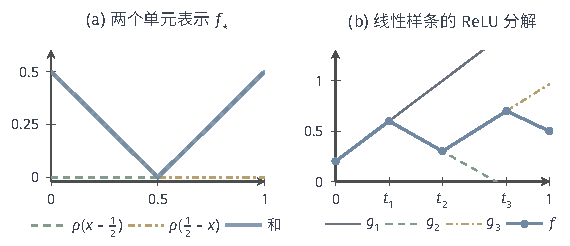
\includegraphics[width=96.6mm]{figures/02-abstract-mathematics/03-function-spaces/tikz/c6-relu-units/figure.pdf}
  \caption{ReLU单元的有限组合。(a)~$\rho(x-\frac12)$与$\rho(\frac12-x)$之和恰为$f_*$。(b)~结点$0,t_1,t_2,t_3,1=0,0.25,0.5,0.8,1$、结点值$0.2,0.6,0.3,0.7,0.5$的线性样条$f$（蓝），按式~\eqref{eq:apx-relu-spline}写成$0.2+1.6\rho(x)-2.8\rho(x-0.25)+\frac{38}{15}\rho(x-0.5)-\frac73\rho(x-0.8)$；细线$g_1,g_2,g_3$依次是前一、二、三个单元的部分和，每加一个单元就在对应结点处改变斜率。}
  \label{fig:apx-relu-units}
\end{figure}

\paragraph{单隐藏层通用逼近定理}

一维构造依赖分段线性的特殊结构。对多维输入和一般激活函数，需要下面的存在定理。

\begin{theorem}[单隐藏层网络的通用逼近]
\label{thm:apx-universal-approximation}
设$X\subset\mathbb R^d$是非空紧集，激活函数$\sigma:\mathbb R\to\mathbb R$连续且不是多项式。则形如
\begin{equation}
  g(\bm x)=\sum_{j=1}^{M}a_j\,\sigma(\bm w_j^{\top}\bm x+b_j),
  \qquad M\in\mathbb N,\ a_j,b_j\in\mathbb R,\ \bm w_j\in\mathbb R^d
  \label{eq:apx-one-hidden-layer}
\end{equation}
的函数全体在$C(X)$中按一致范数稠密。
\end{theorem}

这一形式的结论由Leshno、Lin、Pinkus与Schocken证明\cite{leshno1993approximation}，他们的结果对更广的局部有界、分段连续激活也成立；此前Cybenko对S型激活给出了同类结论\scite{cybenko1989approximation}。这里只陈述并使用连续激活的情形，证明从略。在式~\eqref{eq:apx-one-hidden-layer}外再加一个输出偏置，不改变结论。

定理的条件都可以用例子检查。Sigmoid函数$1/(1+e^{-s})$、$\tanh s$和ReLU都连续且不是多项式，所以都满足条件；定理不要求激活处处可微。

多项式激活必须排除。若$\sigma$是$r$次多项式，则$\sigma(\bm w^{\top}\bm x+b)$是$\bm x$的至多$r$次多项式，无论$M$多大，$g$都落在“$d$元至多$r$次多项式”这个有限维子空间中。若$X$含有内点，函数$x_1^{r+1}$不在这个子空间中；有限维子空间是闭的，所以$x_1^{r+1}$与它的一致距离为正。增加宽度不能增加可表达的次数，“使用了非线性函数”不能代替“非多项式”这一条件。

偏置也不能省略。在$[0,1]$上取ReLU且令所有$b_j=0$，则$\rho(w_jx)$在$w_j>0$时等于$w_jx$，在$w_j\le0$时恒为零，所有组合都形如$cx$。这样的函数在$0$处为零，无法逼近常函数$1$。

\paragraph{表示能力之外的问题}

通用逼近定理断言“存在”一组参数，它不回答以下几个问题，每个都需要单独的条件和论证。

参数不可识别。同一个函数有许多参数表示：交换隐藏单元的次序不改变输出；ReLU的正齐次性给出$a\rho(wx+b)=(a/\lambda)\rho(\lambda wx+\lambda b)$（$\lambda>0$）；在$[0,1]$上还有$f_*(x)=2\rho(x-\frac12)-\rho(x)+\frac12$，它与前面的两单元表示使用不同的单元。因此不能由函数反推出唯一的参数。

寻找参数与推广到新样本是另外的问题。定理不说明梯度方法能否找到逼近参数，也不说明由有限样本训练出的网络在新输入上误差小；相应的分析可参考\BookChapterRef{chap:feedforward-networks}{卷八“前馈神经网络”章}和\BookChapterRef{chap:deep-learning-theory}{卷六“深度学习的可学习性”章}。

评价范数也要说明。若输入服从$X$上的概率测度$\mu$，则$\|f-g\|_{L^2(\mu)}\le\|f-g\|_\infty$，一致逼近自动给出平均意义下的逼近；反方向不成立，一个只在小区域上很高的尖峰可以使$L^2(\mu)$误差很小而一致误差很大。向量值目标可以逐坐标逼近，再把各坐标的隐藏单元并列放进同一隐藏层。
